%%%%%%%%%%%%%%%%%%%%%%%%%%%%%%%%%%%%%%%%%%%%%%%%%%%%%%%%%%%%%%%%%%%%%%%%%%%%%
%
%  System        : 
%  Module        : 
%  Object Name   : $RCSfile$
%  Revision      : $Revision$
%  Date          : $Date$
%  Author        : $Author$
%  Created By    : Robert Heller
%  Created       : Sat Apr 15 10:38:17 2023
%  Last Modified : <230422.1448>
%
%  Description 
%
%  Notes
%
%  History
% 
%%%%%%%%%%%%%%%%%%%%%%%%%%%%%%%%%%%%%%%%%%%%%%%%%%%%%%%%%%%%%%%%%%%%%%%%%%%%%
%
%    Copyright (C) 2023  Robert Heller D/B/A Deepwoods Software
%			51 Locke Hill Road
%			Wendell, MA 01379-9728
%
%    This program is free software; you can redistribute it and/or modify
%    it under the terms of the GNU General Public License as published by
%    the Free Software Foundation; either version 2 of the License, or
%    (at your option) any later version.
%
%    This program is distributed in the hope that it will be useful,
%    but WITHOUT ANY WARRANTY; without even the implied warranty of
%    MERCHANTABILITY or FITNESS FOR A PARTICULAR PURPOSE.  See the
%    GNU General Public License for more details.
%
%    You should have received a copy of the GNU General Public License
%    along with this program; if not, write to the Free Software
%    Foundation, Inc., 675 Mass Ave, Cambridge, MA 02139, USA.
%
% 
%
%%%%%%%%%%%%%%%%%%%%%%%%%%%%%%%%%%%%%%%%%%%%%%%%%%%%%%%%%%%%%%%%%%%%%%%%%%%%%

\subsection{Crossing with interchange}
\label{sect-appl:crossinginterchange}

\begin{figure}[hbpt]\begin{centering}%
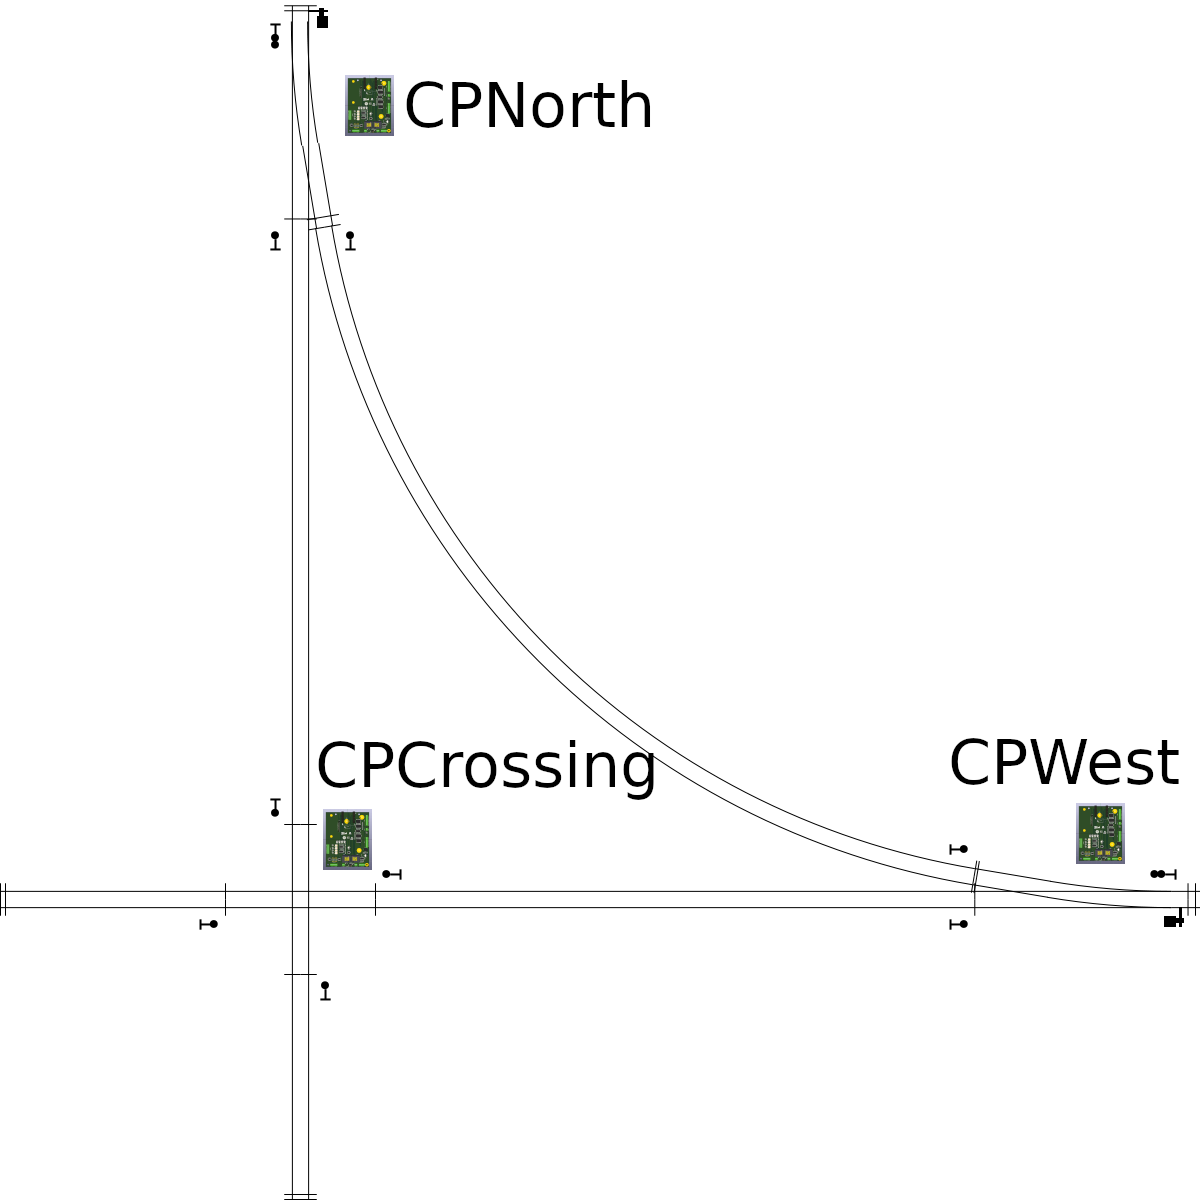
\includegraphics[width=5in]{CrossingInterchange.png}
\caption{Crossing with Interchange.}
\label{fig:CrossingInterchange}
\end{centering}\end{figure}

This is a level crossing with an interchange track.  We will control and 
manage this crossing and interchange with three ESP32 T7S3 MultiFunction 
Universal Turnout nodes, as shown in Figure~\ref{fig:CrossingInterchange}. The 
three nodes will implement these functions:

\begin{description}
\item [CPNorth] This node will manage the north turnout and the signals around 
it.  It will also provide occupancy detection for the turnout OS section and 
the north-south track segment. It will be wired as following:
\begin{description}
\item [OC 1] The turnout OS section.
\item [OC 2] The north-south track segment.
\item [Turnout 1] The north turnout motor.
\item [Points 1] The north turnout points.
\item [A0(UR), A1(UY), A2(UG), A3(LR), A4(LY), A5(LG)] The signal at the north 
(points) end of the turnout.
\item [B0(R), B1(Y), B2(G)] The interchange segment (divergent frog) 
end of the turnout.
\item [B3(R), B4(Y), B5(G)] The north-south track segment 
(non-divergent frog) end of the turnout.
\end{description} 
\item [CPEast] This node will manage the east turnout and the signals 
around it.  It will also provide occupancy detection for the turnout OS 
section, the east-west track segment, and the interchange track segment.  It 
will be wired as following: 
\begin{description}
\item [OC 1] The turnout OS section.
\item [OC 2] The east-west track segment.
\item [OC 3] The interchange track segment
\item [Turnout 1] The west turnout motor.
\item [Points 1] The west turnout points.
\item [A0(UR), A1(UY), A2(UG), A3(LR), A4(LY), A5(LG)] The signal at the west 
(points) end of the turnout.
\item [B0(R), B1(Y), B2(G)] The interchange segment (divergent frog) 
end of the turnout.
\item [B3(R), B4(Y), B5(G)] The east-west track segment 
(non-divergent frog) end of the turnout.
\end{description} 
\item [CPCrossing] This node will manage the crossing diamond, including the 
signals around it along with occupancy detection of the diamond itself.  It 
will be wired as following: 
\begin{description}
\item [OC 1] The east-west part of the crossing.
\item [OC 2] The north-south part of the crossing.
\item [A0(R), A1(Y), A2(G)] The signal at the west end of the crossing.
\item [A3(R), A4(Y), A5(G)] The signal at the east end of the crossing.
\item [B0(R), B1(Y), B2(G)] The signal at the north end of the crossing.
\item [B3(R), B4(Y), B5(G)] The signal at the south end of the crossing.
\end{description}
\end{description}

The CPNorth and CPEast will actually be configured following the much the same 
methods as an end of a siding, as describe in 
Section~\ref{sect-appl:siding}\footnote{The local control buttons and LEDs are
not shown here - they could be added or left out as desired.} Since we are 
using 3 over 3 signals at the points ends of the turnouts, it is possible to 
add additional aspects. 


\begin{figure}[hbpt]\begin{centering}%
\includegraphics[width=5in]{Crossing_CPNorth.pdf}
\caption{CPNorth  Event Id graph.}
\label{fig:CrossingCPNorthEventFlow}
\end{centering}\end{figure}
\begin{figure}[hbpt]\begin{centering}%
\includegraphics[width=5in]{Crossing_CPEast.pdf}
\caption{CPEast  Event Id graph.}
\label{fig:CrossingCPEastEventFlow}
\end{centering}\end{figure}
\begin{figure}[hbpt]\begin{centering}%
\includegraphics[width=5in]{Crossing_CPCrossing.pdf}
\caption{CPCrossing Event Id graph.}
\label{fig:CrossingCPCrossing}
\end{centering}\end{figure}
\clearpage
\begin{table}[hbpt]\begin{centering}%
\begin{tabular}{|l|l|p{2in}|}
\hline
Color&Object&What it is\\
\hline
Orange&Node&Occupancy Detectors\\
\hline
Green&Node&Siding normal button and LED\\
\hline
Red&Node&Siding reversed button and LED\\
\hline
Cyan&Node&Logic Elements\\
\hline
Blue&Node&Turnout Outputs\\
\hline
LightSeaGreen&Node&Point Sense Inputs\\
\hline
RoyalBlue&Node&Masts\\
\hline 
Green&Edge&Button and LED normal Events\\
\hline
Red&Edge&Button and LED reverse Events\\
\hline
Brown&Edge&Button Release Events\\
\hline
Green&Edge&Turnout Operating Events\\
\hline
Black&Edge&Logic Fallthroughs (Elses)\\
\hline
Orange&Edge&Odd Yard Tracks (1 and 3)\\
\hline
Violet&Edge&Even Yard Tracks (2 and 4)\\
\hline
Cyan&Edge&Mast Rule Selection\\
\hline
LightSeaGreen&Edge&Point Sense events\\
\hline
\end{tabular}
\caption{Graph color key}
\label{tab:ExampleSidingCP1EventFlow}
\end{centering}\end{table}


\clearpage
